\documentclass[../Bachelorarbeit.tex]{subfiles}

\begin{document}
\label{sec:EFT}

\begin{figure}[h]
    \centering
    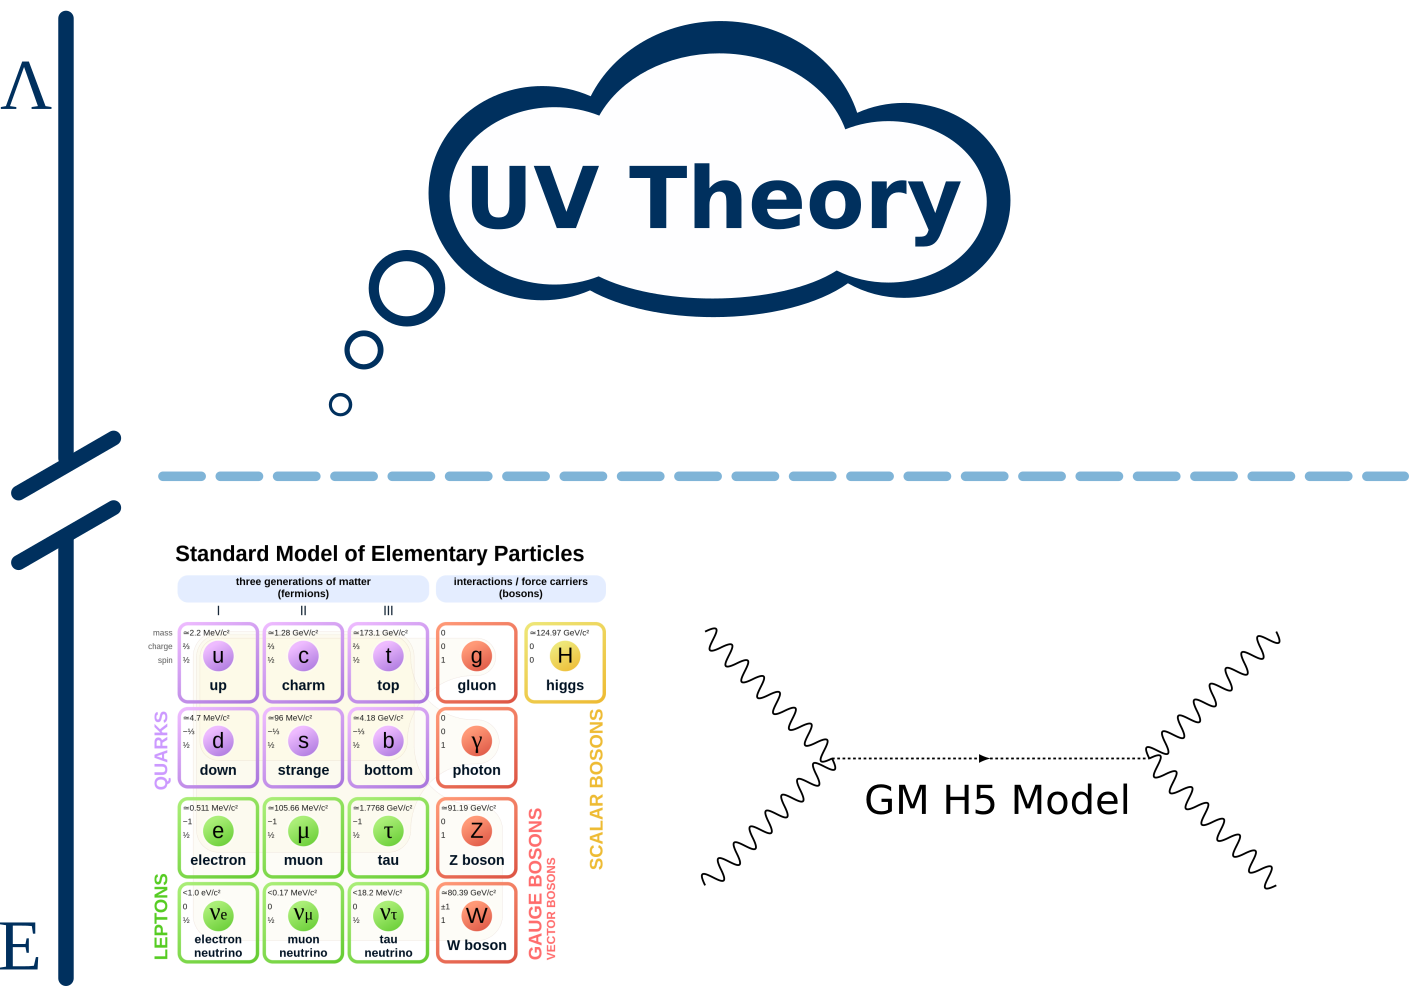
\includegraphics[width=\textwidth]{images/EFT_Model.png}
    \label{fig:EFT_sketch}
    \caption{Source and text \cite{Brivio.2017}}
\end{figure}

With the Standard Model Physicist try to describe the elementary Particles and interactions. It is successful in describing most processes in Biology, Chemistry, and Physics.
But the Standard Model is still incomplete. It can't describe Phenomenons like Gravity, Neutrino Masses, Matter-Antimatter asymmetry etc. This is where effective field theory comes in.
Here we look at the Standard Model as a low energy approximation of an underlying Ultraviolet Theory (figure~\ref{fig:EFT_sketch}).
\\\\
The concept of an Effective Field Theory(EFT) can be Illustrated in different ways using the Euler-Heisenberg Lagrangian, the Fermi theory or the Standard Model Effective Field Theory(EFT).
\cite{Pich.1998} shows The Euler-Heisenberg Lagrangian and the Fermi theory while I will be focusing on the SMEFT, as the Name suggests The SMEFT aims to extant the Standard Model.
Except the g-Faktor of the Myon the Standard Model has been robust without meaningful deviations from Experimental Measurements. 
%With that in mind it is reasonable to assume that new Particles are heavier than Particles within the weak scale. 
%This allows the SMEFT a Model-indepentent way to describe Beyond the Standard Model effects.
There using a theory that keeps the $SU(3) \times SU(2) \times U(1)$ symmetry with the Higgs field breaking gauge symmetry is desirable.
Therefore, we construct the Lagrangian from the gauge invariance for Standard Model fields but allow arbitrarily large mass dimensions. 
With that any SMEFT Lagrangian can be written as:

\begin{equation}
    \mathcal{L}_{SMEFT} = \mathcal{L}_{SM} + \frac{1}{\Lambda} \mathcal{L}_{5} + \frac{1}{\Lambda^2} \mathcal{L}_{6} + \frac{1}{\Lambda^3} \mathcal{L}_{7} + \frac{1}{\Lambda^4} \mathcal{L}_{8} + ... \textnormal{ with } \mathcal{L}_{i} = \sum_{i} c_{i}^{D} \mathcal{O}_{i}^{D}
    \label{eq:L_SMEFT}
\end{equation}

The operators $\mathcal{O}_{i}$ are constructed from the Gauge invariance of the SM fields while the Wilson coefficients $c_{i}$ contain the information on heavy degrees of freedom.
Normally the heavy degrees of freedom are integrated out to have a renomilazible Theory but are needed to describe high energy Particles.
We get the Wilson coefficients from the operator product expansion in \ref{eq:L_SMEFT}. Again a good example for the operator product expansion is the Fermi Theory shown in \cite{Pich.1998}.
For a characteristic heavy scale $\Lambda$ the operators are ordered by there dimension $d_{i}$ fixing the dimension of their respective coefficients.

\begin{equation}
    [\mathcal{O}_i] = d_{i} \longrightarrow c_{i} \sim \frac{1}{\Lambda^{d_{i}-4}}
\end{equation}

The Leading order $D = 4$ term in \ref{eq:L_SMEFT} is the SM Lagrangian while deviations of the SM are described by operators with a dimension $D>4$.



\end{document}
